\section{Data and Resources}

In this paper we investigate methods to estimate Web pages understandability, including the effect HTML preprocessing pipelines and heuristic have, and their search effectiveness when employed within retrieval methods. To obtain both topical relevance and  understandability assessments, we used the data from the CLEF 2015 and 2016 eHealth collections. 

The CLEF 2015 collection contains 50 queries and 1,437 documents have been assessed relevant by clinical experts and have an assessment for understandability~\cite{clef15}. Documents in this collections are a selected crawl of health websites, of which the majority are certified Health on the Net (HON) websites.
The CLEF 2016 collection contains 300 queries and 3,298 relevant documents that also have been assessed with respect to understandability~\cite{clef16}. Documents in this collection belong to the Clueweb12b corpus, and thus are general English Web pages, not necessarily targeted to health topics, nor of a controlled quality (as are instead HON certified sites). 
Understandability assessments were provided on a 5-point Likert scale for CLEF 2015, and within a $[0,100]$ range for CLEF 2016 (0 lowest understandability). 

To support the investigation in Section~\ref{sec:which_preprocessing} (influence of pre-processing on understandability estimation), we further considered correlations between multiple human assessors (inter-assessor agreement). For CLEF 2015, we used the publicly available additional assessments made by unpaid medical students and health consumers collected by Palotti et al.~\cite{palotti16b} in a study of how medical expertise affects assessments. For CLEF 2016 we  collected understandability assessments for 100 documents. Three members of our research team, which did not author this paper, were recruited and instructed to provided the assessments. The Relevantion tool~\cite{} was used to assist with the assessments, mimicking the settings used for the CLEF collections.


In the experiments, we used Pearson, Kendall and Spearman's Rank correlations to compare the understandability assessments of human assessors with estimations obtained with readability formulas, under all combinations of extraction pipelines and sentence-ending heuristics. Pearson correlation is used to calculate the strength of the linear relation between two variables, while the Kendall and Spearman measure the rank correlations between the variables. We opted to report all three correlation coefficients to allow for a thorough comparison to other work, as they are equally used in the literature. 

\todo{move IR measures here}

\todo{link to online appendix for all results}

%\section{Which Readability Formula To Use}
%\section{Influence of Preprocessing on Readability Formulas}
%\label{sec:which_readability}

%Next, we report on our study of the influence of the preprocessing of Web pages on the estimation of understandability when using surface level readability formulas like SMOG, CLI, etc. We did so by comparing the combination of a number of pre-processing pipelines and heuristics and readability formula with human assessments of web page understandability. 
%Our experiments extended those by Palotti et al.~\cite{palotti15}, who did not compare their results against human assessments. 

%We employed the same three approaches used in Palotti et al.~\cite{palotti15} to extract the content of a Web page from the HTML source: BeautifulSoap 4 (\textit{Naive}), which just naively removes HTML tags, Boilerpipe\cite{kohlschutter10} (\textit{Boilerpipe - Boi}) and Justext\cite{jan11} ({Justext - Jst}), which eliminate boilerplate text together with HTML tags. 
%Their data analysis highlighted that the text in HTML tags often missed a correct punctuation mark and thus the text extracted from HTML fields like titles, menus, tables and lists could be interpreted as many short sentences or few very long sentences, depending on whether a period was forced at the end of fields/sentences. We thus implemented the same two heuristics to deal with this: \textit{ForcePeriod - FP} and \textit{DoNotForcePeriod - DNFP}. The \textit{ForcePeriod - FP} heuristics forced a period at the end of each extracted HTML field; while the \textit{DoNotForcePeriod - DNFP} did not. 

%We used Pearson, Kendall and Spearman's Rank correlations to compare the understandability assessments of human assessors with estimations obtained with readability formulas, under all combinations of extraction pipelines and sentence-ending heuristics. Pearson correlation is used to calculate the strength of the linear relation between two variables, while the Kendall and Spearman measure the rank correlations between the variables. We opted to report all three correlation coefficients to allow for a thorough comparison to other work, as they are equally used in the literature. 
%To obtain understandability assessments, we used the data from the CLEF 2015 and 2016 eHealth collections. The CLEF 2015 collection contains 50 queries and 1,437 documents have been assessed relevant by clinical experts and have an assessment for understandability~\cite{clef15}, while the CLEF 2016 collection contains 300 queries and 3,298 relevant documents that also have been assessed with respect to understandability~\cite{clef16}. Understandability assessments were provided on a 5-point Likert scale for CLEF 2015, and within a $[0,100]$ range for CLEF 2016 (0 lowest understandability). 

%Correlations between human assessments and readability formulas, under the different settings of extraction pipelines and heuristics are shown in Figure~\ref{fig:bar_corr_clef15}. We found that the \textit{Naive} preprocessing resulted in the lowest correlations, regardless readability formula and heuristics (although \textit{DoNotForcePeriod} performed better than \textit{ForcePeriod}). Using Justext or Boilerplate resulted in higher correlations with human understandability assessments, and the \textit{ForcePeriod} heuristic was shown to be better than the other. These results confirm the speculations of Palotti et al.~\cite{palotti15}: they found these settings to produce lower variances in understandability estimations and thus hypothesise they were better suited to the task.
%
%Overall, the best results (highest correlations) were obtained by SMOG with \textit{ForcePeriod} and Justext for CLEF 2015 and Dale-Chall Index with \textit{DoNotForcePeriod} and DoNotForcePeriod for CLEF 2016. Although no single setting outperformed the others in both collections, we found that the use of CLI and FRE with \textit{Justext} provided the most stable results across the collections, with correlation coefficients as high as the best ones in both collections.
%
%These results confirm the advice put forward by Palotti et al.~\cite{palotti15}, i.e. if using readability measures, then CLI should be preferred, along with an appropriate HTML extraction pipeline, regardless of the heuristic for sentence ending.


%We observe that the \textit{Naive} preprocessing also results in the lowest
%correlation, no matter which correlation measure or readability formula is used. 

%Also, when the \textit{Naive} preprocessing is used, the variant \textit{DoNotForcePeriod} yields higher correlations than the variant \textit{ForcePeriod}, but when using a higher quality HTML cleaner, such as Justext or Boilerplate, the results indicate that the use of \textit{ForcePeriod} should be preferred.

%Palotti, Zuccon and Hanbury~\cite{palotti15} compared six different HTML cleaning methods and their impact in the use of readability formulas.
%They evaluate three methods to extract the content of a Web page from its HTML source: BeautifulSoap 4, which just naively removed HTML tags, Boilerpipe\cite{kohlschutter10} and Justext\cite{jan11}, two approaches to eliminate boilerplate text together with HTML tags. Henceforth these methods are referred as \textit{Naive}, \textit{Boilerpipe - Boi} and \textit{Justext - Jst}, respectively.
%The authors noticed that the text in HTML tags often missed a correct punctuation mark. For example, the text extract from titles, menus, tables or lists could be interpreted as many short sentences of few very long sentences, depending only whether a period is forced at the end of sentences. These two preprocessing options are henceforth called \textit{ForcePeriod - FP} and \textit{DoNotForcePeriod - DNFP}.

%Their experiments found that the use of \textit{Naive} preprocessing was associated with larger variances in the understandability score estimated by readability formulas, while the use of both \textit{Boi} and \textit{Jst} were more stable. Coleman-Liau Index (CLI) was the most stable metric among all tested in Palotti's work\cite{palotti15}.

%In our experiments, we use the Pearson, Kendall Tau and Spearman's Rank correlation to compare the understandability label assigned to each document by human assessors and by readability formulas.
%Pearson correlation is used to calculate the strength of two linearly related variables, while the Kendall and Spearman are rank correlation, i.e., they act on the rank of the variables instead of their values. We opt to report on all three correlation coefficients as all three are equally used in the literature, and thus we allow other researchers to compare our results across.

%We show in Figure~\ref{fig:bar_corr_clef15} %and~\ref{fig:bar_corr_clef16}
%the correlation scores of each traditional readability metric with the human assessments made in CLEF 2015 and 2016, respectively. We observe that the \textit{Naive} preprocessing also results in the lowest
%correlation, no matter which correlation measure or readability formula is used. Also, when the \textit{Naive} preprocessing is used, the variant \textit{DoNotForcePeriod} yields higher correlations than the variant \textit{ForcePeriod}, but when using a higher quality HTML cleaner, such as Justext or Boilerplate, the results indicate that the use of \textit{ForcePeriod} should be preferred.

%Among all the readability formulas and preprocessing methods, SMOG with \textit{ForcePeriod} preprocessing and Dale-Chall Index with \textit{DoNotForcePeriod} are the best ones respectively for 2015 and 2016. Although there is no single best readability measure or best preprocessing strategy in all scenarios, CLI and FRE with \textit{Justext} are stable options, with correlation coefficients as high as the best ones in both campaigns. Thus, we confirm Palotti's advice for the use of CLI, as it has shown once more to be the most robust measure to variances due to use of \textit{ForcePeriod} or \textit{DoNotForcePerid}.


%\begin{figure*}[th!]
%   \centering
%   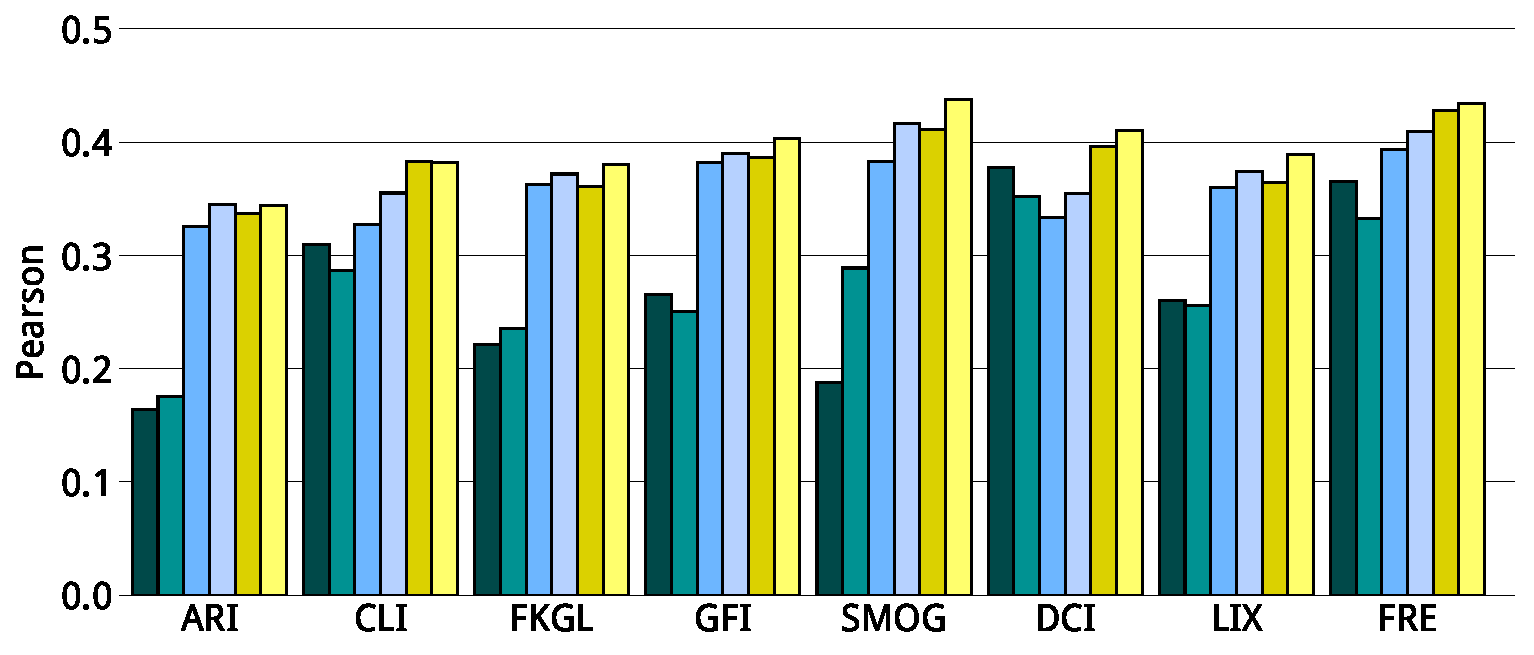
\includegraphics[width=.45\textwidth]{graphics/bar_corr_pearson15_values}
%   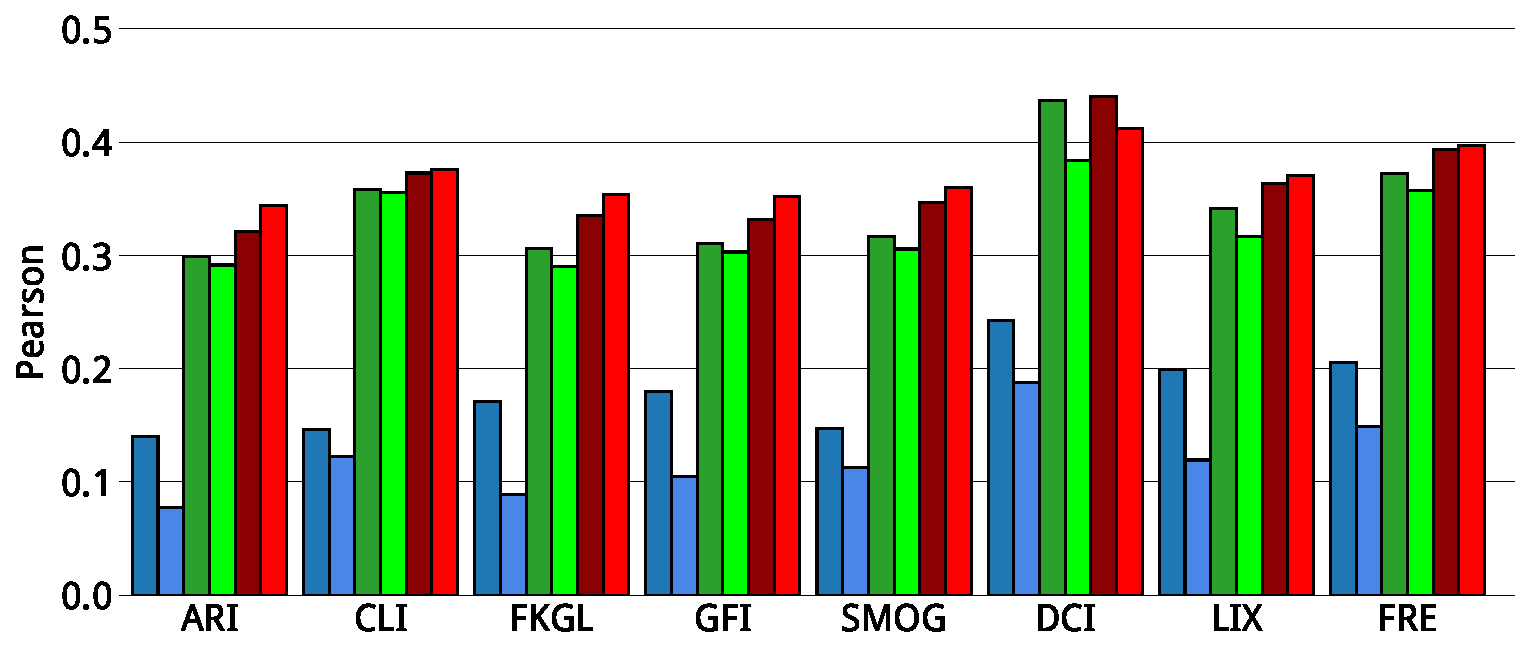
\includegraphics[width=.45\textwidth]{graphics/bar_corr_pearson16_values}
%   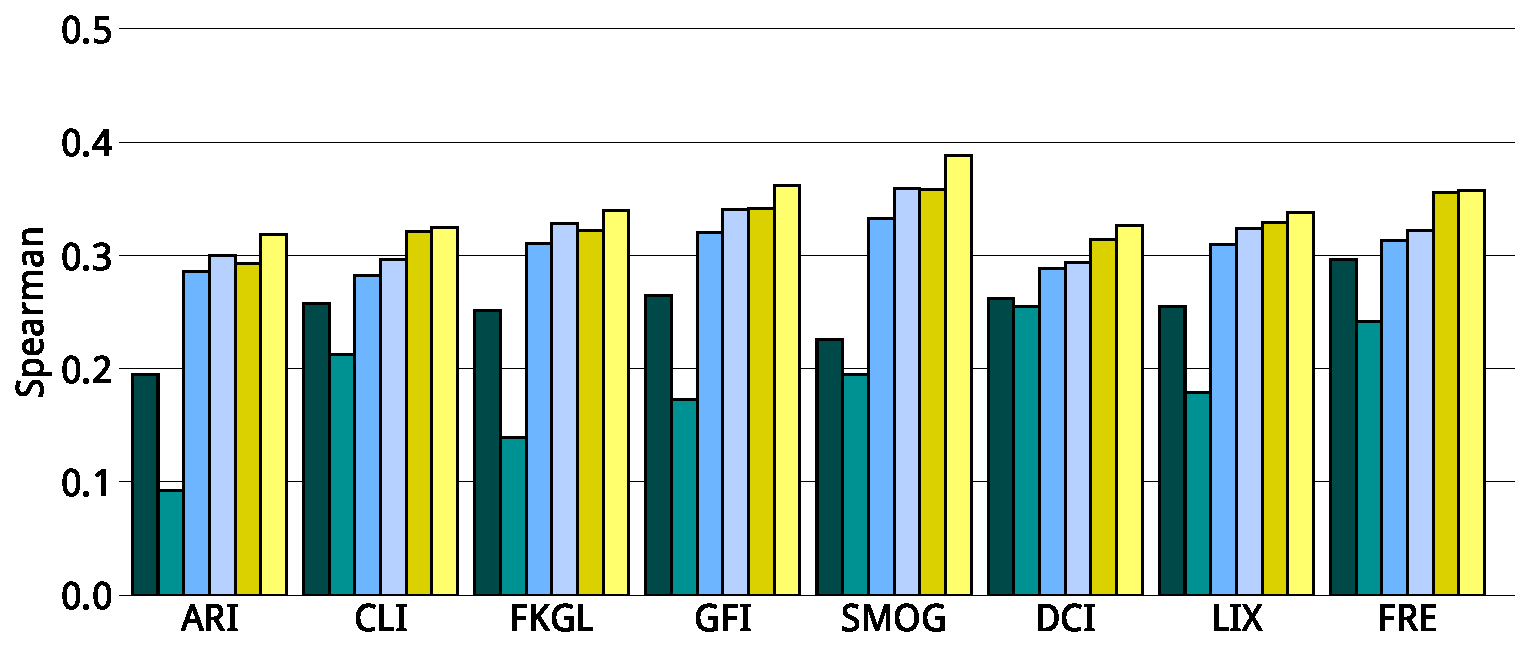
\includegraphics[width=.45\textwidth]{graphics/bar_corr_spearman15_values}
%   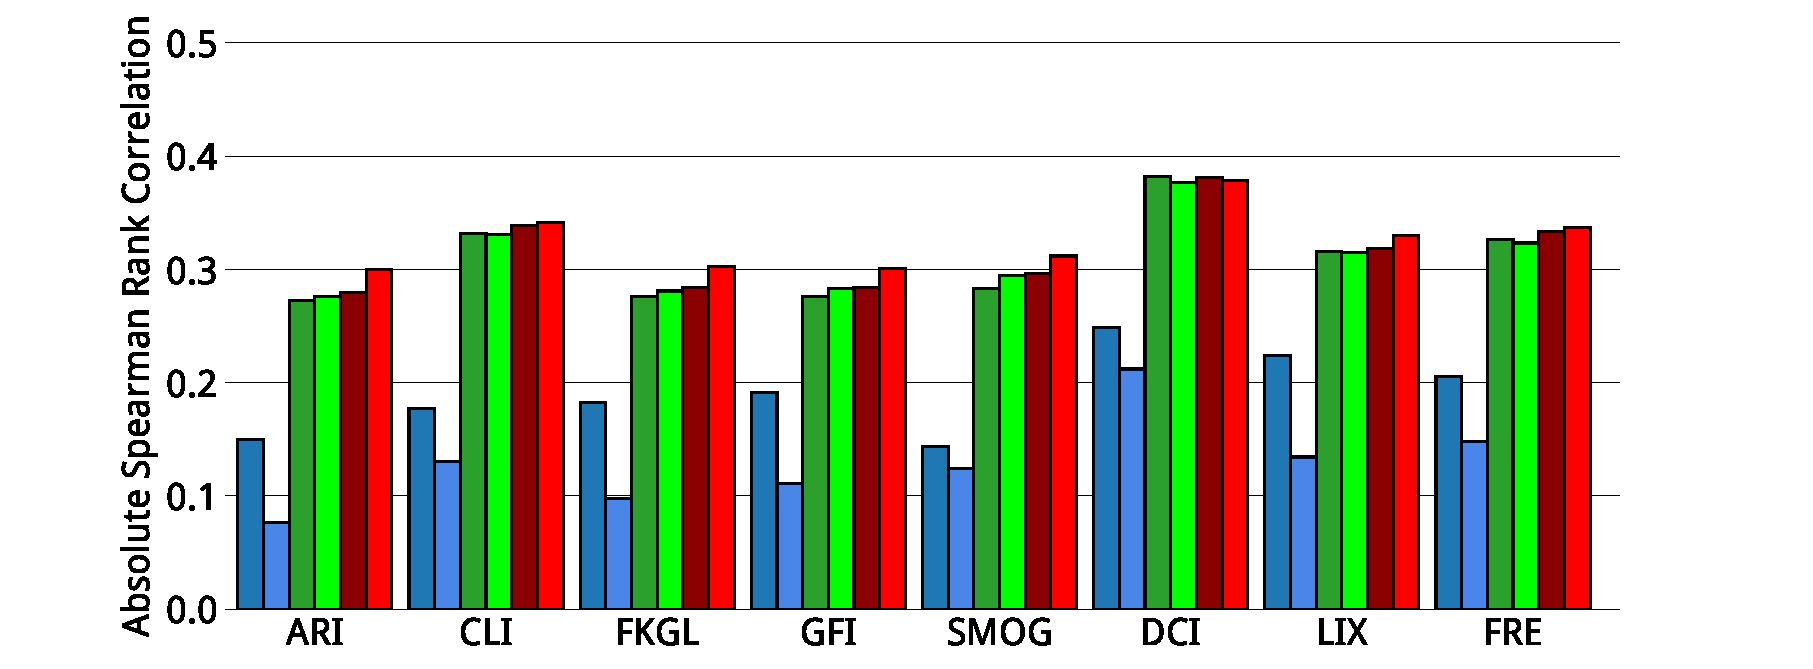
\includegraphics[width=.45\textwidth]{graphics/bar_corr_spearman16_values}
%   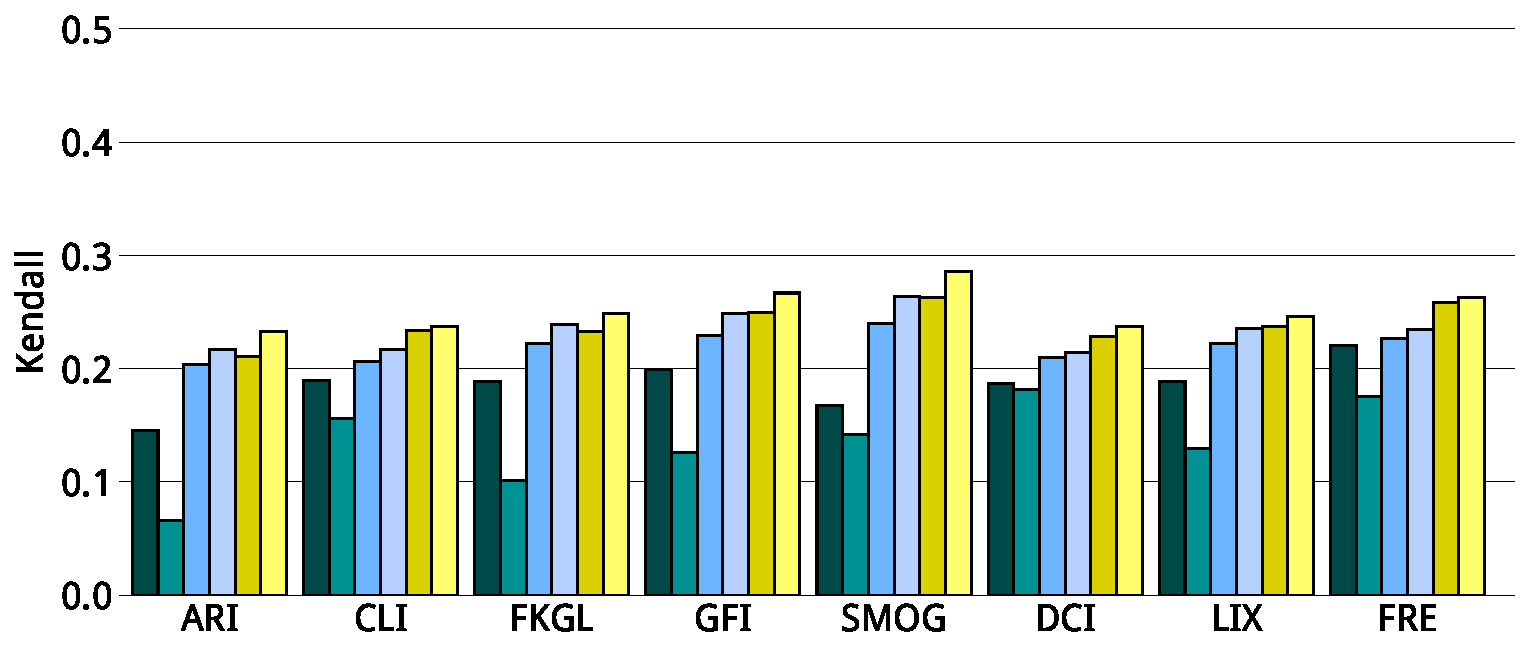
\includegraphics[width=.45\textwidth]{graphics/bar_corr_kendalltau15_values}
%   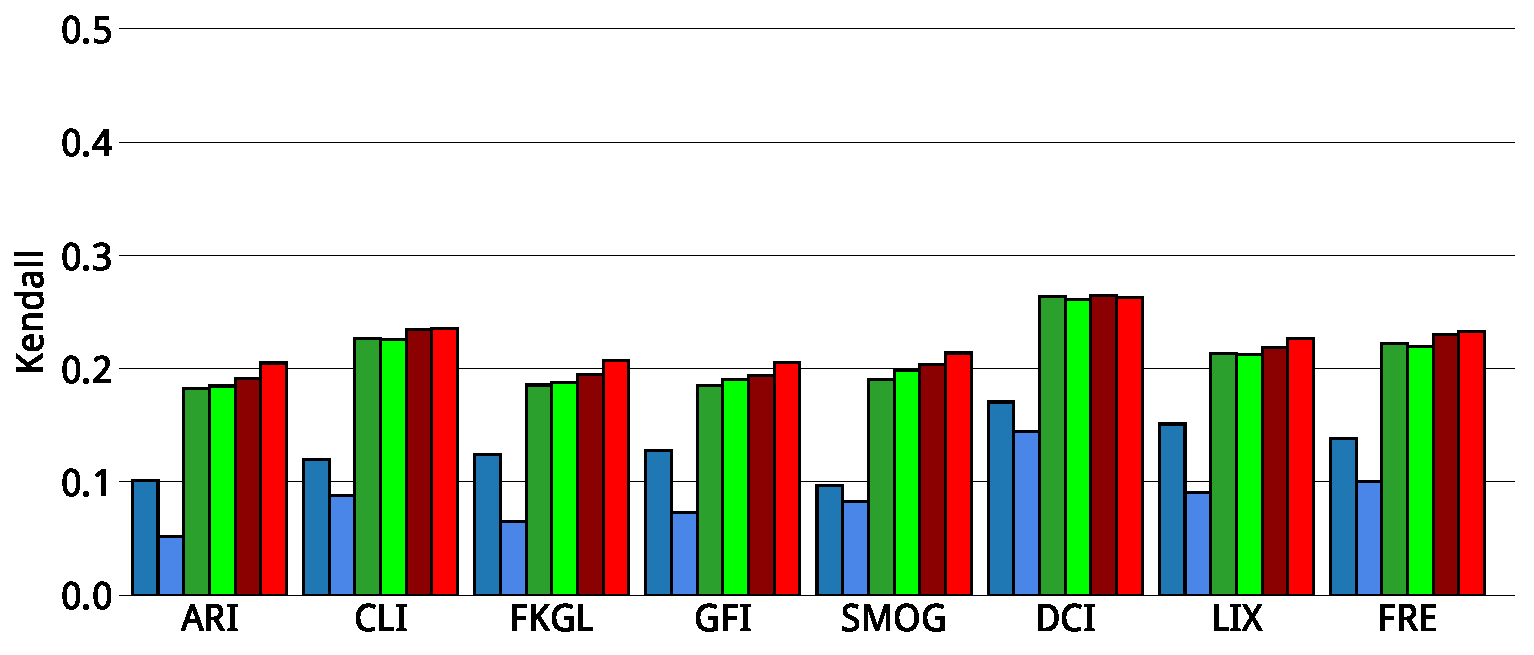
\includegraphics[width=.45\textwidth]{graphics/bar_corr_kendalltau16_values}
%   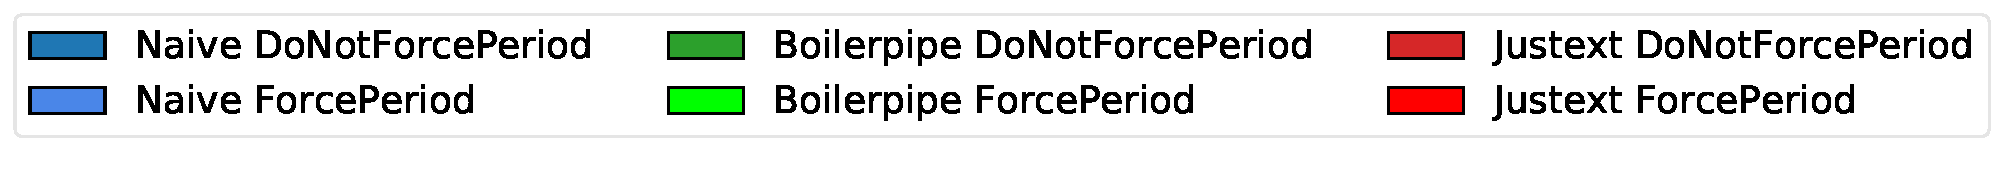
\includegraphics[width=.8\textwidth]{graphics/legend62}
%    \caption{Absolute correlation coefficient of different readability measures and understandability scores. On the left hard side, CLEF eHealth 2015, on the right hand side, CLEF eHealth 2016}
%   \label{fig:bar_corr_clef15}
%\end{figure*}

%\begin{figure*}[th!]
%  \centering
%   \caption{Correlation of different readability measures and the understandability scores collected in CLEF eHealth 2016.}
%  \label{fig:bar_corr_clef16}
%\end{figure*}


